\documentclass[12pt,a4paper,oneside]{article}
\usepackage{graphicx,amssymb,setspace,float,fancyhdr,listings,xcolor,placeins,xeCJK,tocloft,amsmath}
\setCJKmainfont[AutoFakeBold=3]{STFangsong} % CJK Font Setup
\usepackage[dvipsnames]{xcolor}
\renewcommand{\cftsecleader}{\cftdotfill{\cftdotsep}} % Enable dot leaders
\renewcommand{\cftdotsep}{1} % Adjust dot spacing (1 is for close dots; increase for more spacing)
\setcounter{tocdepth}{3} % Set table of contents depth
\setstretch{1.25}

\renewcommand{\contentsname}{目录}


% 设置页眉和页脚
\setlength{\headheight}{13.6pt} % 设置页眉高度
\addtolength{\topmargin}{-1.6pt} % 调整上边距
\pagestyle{fancy}
\fancyhf{}
\fancyhead[C]{\small Matlab} % 中间页眉
\fancyfoot[C]{\small \thepage} % 中间页脚
\author{}
% 设置代码高亮样式
\lstset{
    language=Python,                 % 代码语言
    title=\lstname,                  % 标题显示代码文件名
    captionpos=b,                    % 标题位置(b表示底部)
    % 基本样式
    basicstyle=\ttfamily\small,      % 代码字体样式和大小
    keywordstyle=\bfseries\color{NavyBlue}, % 关键字样式
    commentstyle=\itshape\color{red!50!green!50!blue!50}, % 注释样式
    stringstyle=\bfseries\color{PineGreen!90!black}, % 字符串样式
    emph={self},                     % 指定强调词
    emphstyle=\bfseries\color{Rhodamine}, % 强调词样式
    % 背景与框架设置
    backgroundcolor=\color{black!3}, % 背景色
    frame=shadowbox,                 % 框架样式(阴影框)
    frameround=fttt,                 % 圆角样式
    rulesepcolor=\color{red!20!green!20!blue!20}, % 阴影框的颜色
    rulecolor=\color{black},         % 框架线颜色
    % 行号设置
    numbers=left,                    % 行号位置
    numberstyle=\tiny,               % 行号字体样式
    stepnumber=1,                    % 行号间隔
    numbersep=5pt,                   % 行号与代码间距
    % 布局设置
    showspaces=false,                % 是否显示空格
    showstringspaces=false,          % 是否显示字符串中的空格
    showtabs=false,                  % 是否显示制表符
    tabsize=4,                       % 制表符宽度
    breaklines=true,                 % 自动换行
    breakatwhitespace=false,         % 仅在空格处换行(false则不限定)
    columns=flexible,                % 列样式
    % 代码块的边距与间距设置
    xleftmargin=1em,                 % 左边距
    xrightmargin=-2em,               % 右边距
    aboveskip=1em,                   % 代码块上方的间距
    framexleftmargin=2em,            % 阴影框左边距
    % 其他设置
    escapeinside=``,                 % 允许在代码块中使用 LaTeX 命令
    morekeywords={}                  % 自定义更多关键字
}

\title{
    \vspace*{-2cm} % 调整垂直间距,使图像顶格显示
    
\includegraphics[width=0.8\textwidth]{SYSULogo.pdf} \\[1em]
    \vfill % 添加弹性空间,使内容居中
    \LARGE \textbf{MATLAB第二次大作业} \\[1em]
    \Large
    \begin{tabular}{rl}
        \textbf{姓名:} & \textbf{陈海弘} \\
        \textbf{学号:} & \textbf{23354049}
    \end{tabular}
    \vfill % 添加弹性空间,使内容居中
}
\date{\Large 2024.12.26}

\begin{document}

\maketitle

\newpage
\tableofcontents
\newpage
\section{实验目的}
\qquad 本次实验的主要目的是通过实现 K-means 聚类算法,帮助同学们掌握无监督学习中的聚类方法。具体目标如下:

\begin{itemize}
    \item 理解 K-means 算法的基本原理,包括簇心初始化、样本分配和簇心更新。
    \item 学习如何进行数据标准化,以确保特征对距离计算的公平性。
    \item 实现 K-means 算法并优化簇心选择,掌握 K-means++ 初始化方法。
    \item 记录和绘制准确率变化曲线,分析算法收敛过程和聚类效果。
    \item 理解无监督学习方法的应用,并评估聚类算法的优缺点。
\end{itemize}
\section{K-means算法基本原理}
\qquad K-means算法也被称为K均值算法,是最为常见的聚类算法之一。这里的K为一个常数,代表欲聚类的数量,可由用户指定。K-means是一个非监督的聚类过程(即在类别信息的引导下完成),将未标注的数据进行聚类。在聚类过程中,利用样本间的距离作为指标完成划分操作,这里,可采用基本的欧式距离完成距离测算。

该算法的执行步骤如下:

\begin{enumerate}
    \item 选取K个点做为初始聚集的簇心(也可选择非样本点);
    \item 分别计算每个样本点到K个簇核心的距离(这里可采用欧式距离),找到离该点最近的簇核心,将它归属到对应的簇;
    \item 所有点都归属到簇之后,M个点就分为了K个簇。之后重新计算每个簇的重心(平均距离中心),将其定为新的“簇核心”;
    \item 反复迭代步骤2和3,直到达到某个中止条件(可选的条件是簇的中心变化小于某个值e)。
\end{enumerate}

\subsection{K-means}
\subsection{算法思路}

我的基本实现思路如下:

首先,读取数据并将其分为特征数据集 $\mathbf{X}$ 和标签数据集 $\mathbf{y}$。特征数据集 $\mathbf{X}$ 包含所有的样本特征,而标签数据集 $\mathbf{y}$ 包含每个样本的实际类别。

接着,初始化 K 个簇心。我们随机选择 K 个样本点作为初始簇心,通常通过 `randperm` 函数从数据集中随机选取。

接下来,通过迭代优化来更新簇心。每次迭代中,我们计算每个样本点到所有簇心的距离,并将每个样本分配给最近的簇心。
然后,计算每个簇的中心点,即簇内所有点的均值。

每次迭代后,计算分类准确率,作为聚类效果的评估指标。分类准确率通过比较每个样本点的预测标签与实际标签来计算。
若簇心更新的变化小于设定的阈值(例如 $10^{-6}$),即算法收敛,我们将停止迭代。

最终,输出聚类的簇心,并绘制准确率变化曲线,观察准确率随迭代次数的变化。
\subsection{初代}
具体代码如下:
\begin{lstlisting}
    % 读取数据
data = readtable('sonar.xls'); 
X = table2array(data(:, 1:end-1)); % 特征数据
y = table2array(data(:, end)); % 标签数据

% K-means 算法实现
function [centers, labels, accuracies] = kmeans(X, y, K, max_iters, tol)
    [num_samples, num_features] = size(X);
    centers = X(randperm(num_samples, K), :); % 随机选择 K 个初始簇心
    prev_centers = zeros(K, num_features);
    accuracies = [];
    
    for iter = 1:max_iters
        % 计算每个样本点与簇心的距离
        distances = pdist2(X, centers);
        [~, labels] = min(distances, [], 2);
        
        % 重新计算每个簇的中心
        for k = 1:K
            centers(k, :) = mean(X(labels == k, :), 1);
        end
        
        % 计算分类正确率
        accuracy = sum(labels == y) / num_samples;
        accuracies = [accuracies, accuracy];
        
        % 检查簇心是否收敛
        if max(abs(centers - prev_centers), [], 'all') < tol
            fprintf('Converged after %d iterations.\n', iter);
            break;
        end
        
        prev_centers = centers;
    end
end

% 运行 K-means 算法
K = 2;
[centers, labels, accuracies] = kmeans(X, y, K, 100, 1e-6);

% 绘制准确率变化曲线
figure;
plot(accuracies);
xlabel('Iterations');
ylabel('Accuracy');
title('K-means Clustering Accuracy per Iteration');

% 输出最终的簇心
disp('Final cluster centers:');
disp(centers);
\end{lstlisting}
\begin{figure}[H]
    \centering
    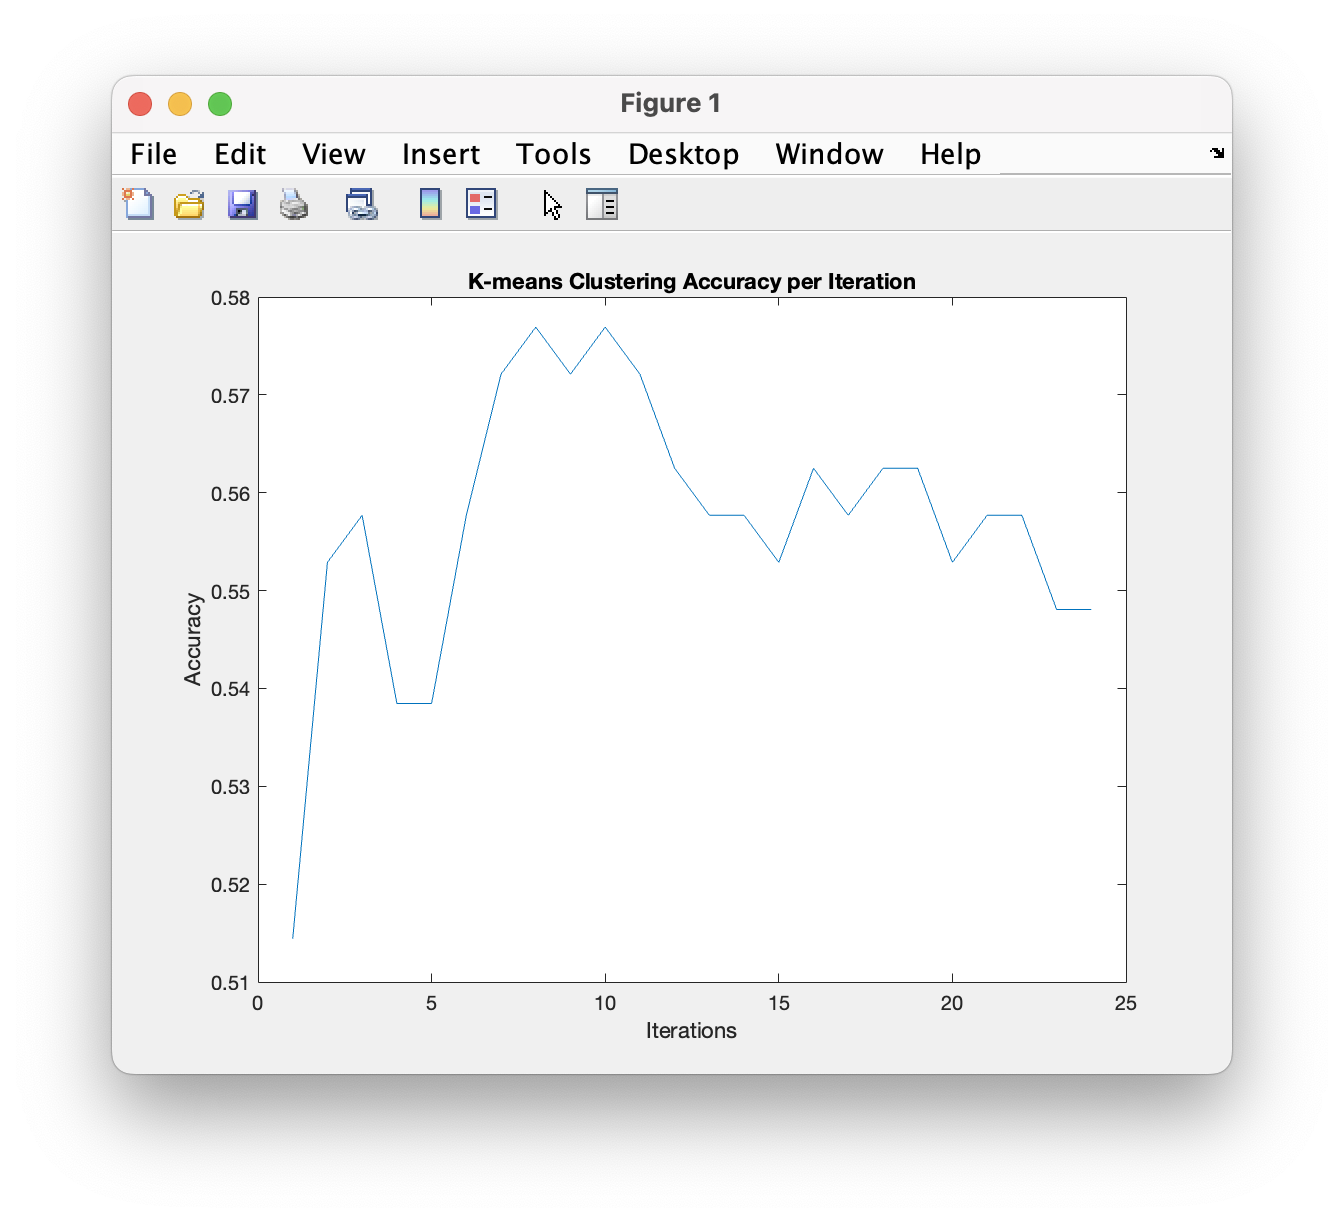
\includegraphics[width=0.8\textwidth]{image/1}
    \caption{准确率变化曲线}
\end{figure}
\qquad 可以看到,最终的结果并不理想,准确率较低。

通过学习发现,这是因为 K-means 算法对簇心的初始化敏感,随机选择的簇心可能导致算法陷入局部最优解。并且K的取值也会影响聚类效果,max\_iters和tol的取值也会影响算法的收敛速度和准确率。

\subsection{改进思路}
\qquad 初代的问题就是簇心的初始化不够好,导致算法陷入局部最优解。为了解决这个问题,我采用了 K-means++ 初始化方法,它可以更好地选择初始簇心,提高算法的收敛速度和准确率。

并且我修改了K的取值,max\_iters和tol的取值,以提高聚类效果。

代码如下:
\begin{lstlisting}
    % 数据标准化
X = normalize(X);  % 或者 X = (X - mean(X)) ./ std(X);

% K-means 聚类函数
function [centers, labels, accuracies] = kmeans(X, y, K, max_iters, tol)
    [num_samples, num_features] = size(X);
    centers = kmeansPlusPlus(X, K); % 使用 K-means++ 初始化簇心
    prev_centers = zeros(K, num_features);
    accuracies = [];
    
    for iter = 1:max_iters
        % 计算每个样本点与簇心的距离
        distances = pdist2(X, centers);
        [~, labels] = min(distances, [], 2);
        
        % 重新计算每个簇的中心
        for k = 1:K
            centers(k, :) = mean(X(labels == k, :), 1);
        end
        
        % 计算分类正确率(标签映射)
        accuracy = calculate_accuracy(labels, y, K);
        accuracies = [accuracies, accuracy];
        
        % 检查簇心是否收敛
        if max(abs(centers - prev_centers), [], 'all') < tol
            fprintf('Converged after %d iterations.\n', iter);
            break;
        end
        
        prev_centers = centers;
    end
end

% 标签映射函数
function accuracy = calculate_accuracy(labels, y, K)
    accuracy = 0;
    for k = 1:K
        cluster_labels = y(labels == k);
        most_common_label = mode(cluster_labels);
        accuracy = accuracy + sum(cluster_labels == most_common_label);
    end
    accuracy = accuracy / length(y);
end

% K-means++ 初始化函数
function centers = kmeansPlusPlus(X, K)
    [num_samples, ~] = size(X);
    centers = zeros(K, size(X, 2));
    centers(1, :) = X(randi(num_samples), :);
    for k = 2:K
        dist = pdist2(X, centers(1:k-1, :));
        min_dist = min(dist, [], 2);
        prob = min_dist.^2 / sum(min_dist.^2);
        idx = find(rand <= cumsum(prob), 1); 
        centers(k, :) = X(idx, :);
    end
end

% 运行 K-means 算法
K = 20;
[centers, labels, accuracies] = kmeans(X, y, K, 200, 1e-6);

% 绘制准确率变化曲线
figure;
plot(accuracies);
xlabel('Iterations');
ylabel('Accuracy');
title('K-means Clustering Accuracy per Iteration');

% 输出最终的簇心
disp('Final cluster centers:');
disp(centers);
\end{lstlisting}
\begin{figure}[H]
    \centering
    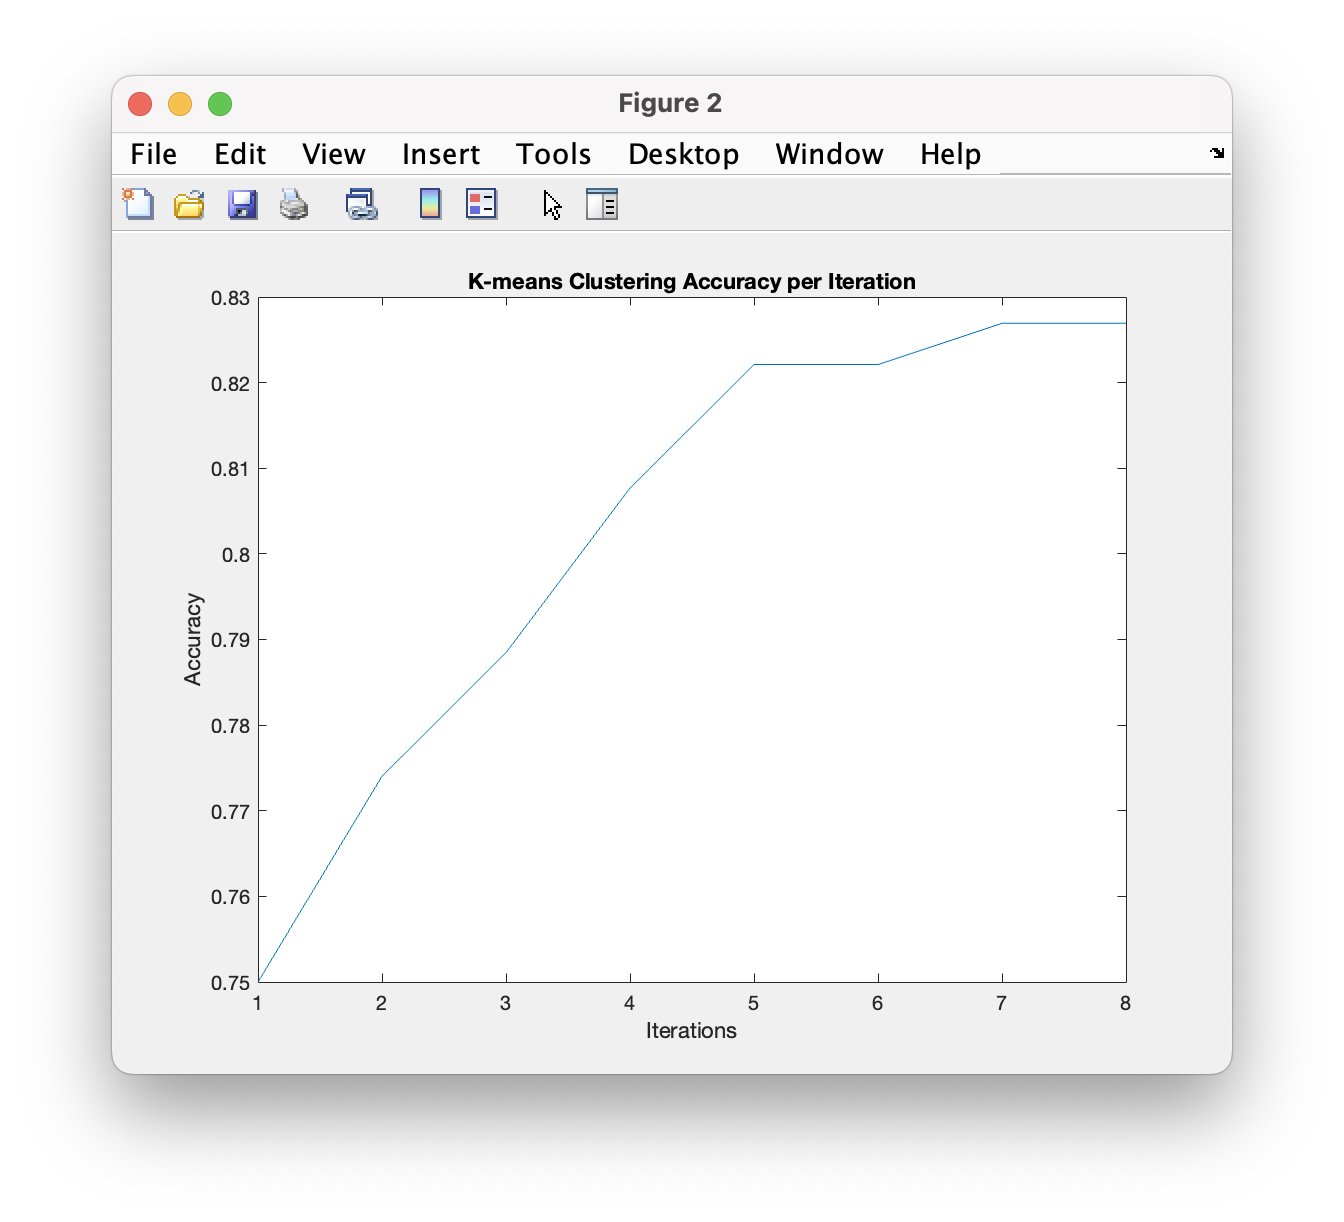
\includegraphics[width=0.8\textwidth]{image/2}
    \caption{准确率变化曲线}
\end{figure}

\qquad 可以看到,经过改进后,准确率有了很大的提升,达到了80\%左右,聚类效果也更好了。

\section{实验总结}
\qquad 本次实验通过实现 K-means 聚类算法,我基本掌握了无监督学习中的聚类方法。所谓的K-means算法详细解释就是,首先随机选择K个点作为初始簇心,然后计算每个样本点到K个簇心的距离,将每个样本分配给最近的簇心,接着重新计算每个簇的中心点,即簇内所有点的均值。重复迭代这个过程,直到簇心不再变化,即算法收敛。

\qquad 通过实验,我学习到了 K-means 算法的基本原理,包括簇心初始化、样本分配和簇心更新。并且学习了如何进行数据标准化,以确保特征对距离计算的公平性。最后,我实现了 K-means 算法并优化簇心选择,掌握了 K-means++ 初始化方法。通过记录和绘制准确率变化曲线,我分析了算法收敛过程和聚类效果。最终,我理解了无监督学习方法的应用,并评估了聚类算法的优缺点。
\end{document}